\documentclass[11pt,compress,t,notes=noshow, xcolor=table]{beamer}
\documentclass[11pt,compress,t,notes=noshow, xcolor=table]{beamer}
\usepackage[]{graphicx}\usepackage[]{color}
% maxwidth is the original width if it is less than linewidth
% otherwise use linewidth (to make sure the graphics do not exceed the margin)
\makeatletter
\def\maxwidth{ %
  \ifdim\Gin@nat@width>\linewidth
    \linewidth
  \else
    \Gin@nat@width
  \fi
}
\makeatother

\definecolor{fgcolor}{rgb}{0.345, 0.345, 0.345}
\newcommand{\hlnum}[1]{\textcolor[rgb]{0.686,0.059,0.569}{#1}}%
\newcommand{\hlstr}[1]{\textcolor[rgb]{0.192,0.494,0.8}{#1}}%
\newcommand{\hlcom}[1]{\textcolor[rgb]{0.678,0.584,0.686}{\textit{#1}}}%
\newcommand{\hlopt}[1]{\textcolor[rgb]{0,0,0}{#1}}%
\newcommand{\hlstd}[1]{\textcolor[rgb]{0.345,0.345,0.345}{#1}}%
\newcommand{\hlkwa}[1]{\textcolor[rgb]{0.161,0.373,0.58}{\textbf{#1}}}%
\newcommand{\hlkwb}[1]{\textcolor[rgb]{0.69,0.353,0.396}{#1}}%
\newcommand{\hlkwc}[1]{\textcolor[rgb]{0.333,0.667,0.333}{#1}}%
\newcommand{\hlkwd}[1]{\textcolor[rgb]{0.737,0.353,0.396}{\textbf{#1}}}%
\let\hlipl\hlkwb

\usepackage{framed}
\makeatletter
\newenvironment{kframe}{%
 \def\at@end@of@kframe{}%
 \ifinner\ifhmode%
  \def\at@end@of@kframe{\end{minipage}}%
  \begin{minipage}{\columnwidth}%
 \fi\fi%
 \def\FrameCommand##1{\hskip\@totalleftmargin \hskip-\fboxsep
 \colorbox{shadecolor}{##1}\hskip-\fboxsep
     % There is no \\@totalrightmargin, so:
     \hskip-\linewidth \hskip-\@totalleftmargin \hskip\columnwidth}%
 \MakeFramed {\advance\hsize-\width
   \@totalleftmargin\z@ \linewidth\hsize
   \@setminipage}}%
 {\par\unskip\endMakeFramed%
 \at@end@of@kframe}
\makeatother

\definecolor{shadecolor}{rgb}{.97, .97, .97}
\definecolor{messagecolor}{rgb}{0, 0, 0}
\definecolor{warningcolor}{rgb}{1, 0, 1}
\definecolor{errorcolor}{rgb}{1, 0, 0}
\newenvironment{knitrout}{}{} % an empty environment to be redefined in TeX

\usepackage{alltt}
\newcommand{\SweaveOpts}[1]{}  % do not interfere with LaTeX
\newcommand{\SweaveInput}[1]{} % because they are not real TeX commands
\newcommand{\Sexpr}[1]{}       % will only be parsed by R
\newcommand{\xmark}{\ding{55}}%


\usepackage[english]{babel}
\usepackage[utf8]{inputenc}

\usepackage{dsfont}
\usepackage{verbatim}
\usepackage{amsmath}
\usepackage{amsfonts}
\usepackage{amssymb}
\usepackage{bm}
\usepackage{csquotes}
\usepackage{multirow}
\usepackage{longtable}
\usepackage{booktabs}
\usepackage{enumerate}
\usepackage[absolute,overlay]{textpos}
\usepackage{psfrag}
\usepackage{algorithm}
\usepackage{algpseudocode}
\usepackage{eqnarray}
\usepackage{arydshln}
\usepackage{tabularx}
\usepackage{placeins}
\usepackage{tikz}
\usepackage{setspace}
\usepackage{colortbl}
\usepackage{mathtools}
\usepackage{wrapfig}
\usepackage{bm}
\usepackage{amsmath}
\usepackage{pifont}

\usetikzlibrary{shapes,arrows,automata,positioning,calc,chains,trees, shadows}
\tikzset{
  %Define standard arrow tip
  >=stealth',
  %Define style for boxes
  punkt/.style={
    rectangle,
    rounded corners,
    draw=black, very thick,
    text width=6.5em,
    minimum height=2em,
    text centered},
  % Define arrow style
  pil/.style={
    ->,
    thick,
    shorten <=2pt,
    shorten >=2pt,}
}

\usepackage{subfig}

% Defines macros and environments
\usepackage{../../style/lmu-lecture}


\let\code=\texttt
\let\proglang=\textsf

\setkeys{Gin}{width=0.9\textwidth}

\setbeamertemplate{frametitle}{\expandafter\uppercase\expandafter\insertframetitle}

% This file is included in slides and exercises

% Rarely used fontstyle for R packages, used only in 
% - forests/slides-forests-benchmark.tex
% - exercises/single-exercises/methods_l_1.Rnw
% - slides/cart/attic/slides_extra_trees.Rnw
\newcommand{\pkg}[1]{{\fontseries{b}\selectfont #1}}

% Spacing helpers, used often (mostly in exercises for \dlz)
\newcommand{\lz}{\vspace{0.5cm}} % vertical space (used often in slides)
\newcommand{\dlz}{\vspace{1cm}}  % double vertical space (used often in exercises, never in slides)
\newcommand{\oneliner}[1] % Oneliner for important statements, used e.g. in iml, algods
{\begin{block}{}\begin{center}\begin{Large}#1\end{Large}\end{center}\end{block}}

% Don't know if this is used or needed, remove?
% textcolor that works in mathmode
% https://tex.stackexchange.com/a/261480
% Used e.g. in forests/slides-forests-bagging.tex
% [...] \textcolor{blue}{\tfrac{1}{M}\sum^M_{m} [...]
% \makeatletter
% \renewcommand*{\@textcolor}[3]{%
%   \protect\leavevmode
%   \begingroup
%     \color#1{#2}#3%
%   \endgroup
% }
% \makeatother






% latex-math includes as needed
% dependencies: amsmath, amssymb, dsfont
% math spaces
\ifdefined\N
\renewcommand{\N}{\mathds{N}} % N, naturals
\else \newcommand{\N}{\mathds{N}} \fi
\newcommand{\Z}{\mathds{Z}} % Z, integers
\newcommand{\Q}{\mathds{Q}} % Q, rationals
\newcommand{\R}{\mathds{R}} % R, reals
\ifdefined\C
\renewcommand{\C}{\mathds{C}} % C, complex
\else \newcommand{\C}{\mathds{C}} \fi
\newcommand{\continuous}{\mathcal{C}} % C, space of continuous functions
\newcommand{\M}{\mathcal{M}} % machine numbers
\newcommand{\epsm}{\epsilon_m} % maximum error

% counting / finite sets
\newcommand{\setzo}{\{0, 1\}} % set 0, 1
\newcommand{\setmp}{\{-1, +1\}} % set -1, 1
\newcommand{\unitint}{[0, 1]} % unit interval

% basic math stuff
\newcommand{\xt}{\tilde x} % x tilde
\newcommand{\argmin}{\mathop{\mathrm{arg\,min}}} % argmin
\newcommand{\argmax}{\mathop{\mathrm{arg\,max}}} % argmax
\newcommand{\argminlim}{\argmin\limits} % argmin with limits
\newcommand{\argmaxlim}{\argmax\limits} % argmax with limits
\newcommand{\sign}{\operatorname{sign}} % sign, signum
\newcommand{\I}{\mathbb{I}} % I, indicator
\newcommand{\order}{\mathcal{O}} % O, order
\newcommand{\bigO}{\mathcal{O}} % Big-O Landau
\newcommand{\littleo}{{o}} % Little-o Landau
\newcommand{\pd}[2]{\frac{\partial{#1}}{\partial #2}} % partial derivative
\newcommand{\floorlr}[1]{\left\lfloor #1 \right\rfloor} % floor
\newcommand{\ceillr}[1]{\left\lceil #1 \right\rceil} % ceiling
\newcommand{\indep}{\perp \!\!\! \perp} % independence symbol

% sums and products
\newcommand{\sumin}{\sum\limits_{i=1}^n} % summation from i=1 to n
\newcommand{\sumim}{\sum\limits_{i=1}^m} % summation from i=1 to m
\newcommand{\sumjn}{\sum\limits_{j=1}^n} % summation from j=1 to p
\newcommand{\sumjp}{\sum\limits_{j=1}^p} % summation from j=1 to p
\newcommand{\sumik}{\sum\limits_{i=1}^k} % summation from i=1 to k
\newcommand{\sumkg}{\sum\limits_{k=1}^g} % summation from k=1 to g
\newcommand{\sumjg}{\sum\limits_{j=1}^g} % summation from j=1 to g
\newcommand{\summM}{\sum\limits_{m=1}^M} % summation from m=1 to M
\newcommand{\meanin}{\frac{1}{n} \sum\limits_{i=1}^n} % mean from i=1 to n
\newcommand{\meanim}{\frac{1}{m} \sum\limits_{i=1}^m} % mean from i=1 to n
\newcommand{\meankg}{\frac{1}{g} \sum\limits_{k=1}^g} % mean from k=1 to g
\newcommand{\meanmM}{\frac{1}{M} \sum\limits_{m=1}^M} % mean from m=1 to M
\newcommand{\prodin}{\prod\limits_{i=1}^n} % product from i=1 to n
\newcommand{\prodkg}{\prod\limits_{k=1}^g} % product from k=1 to g
\newcommand{\prodjp}{\prod\limits_{j=1}^p} % product from j=1 to p

% linear algebra
\newcommand{\one}{\bm{1}} % 1, unitvector
\newcommand{\zero}{\mathbf{0}} % 0-vector
\newcommand{\id}{\bm{I}} % I, identity
\newcommand{\diag}{\operatorname{diag}} % diag, diagonal
\newcommand{\trace}{\operatorname{tr}} % tr, trace
\newcommand{\spn}{\operatorname{span}} % span
\newcommand{\scp}[2]{\left\langle #1, #2 \right\rangle} % <.,.>, scalarproduct
\newcommand{\mat}[1]{\begin{pmatrix} #1 \end{pmatrix}} % short pmatrix command
\newcommand{\Amat}{\mathbf{A}} % matrix A
\newcommand{\Deltab}{\mathbf{\Delta}} % error term for vectors

% basic probability + stats
\renewcommand{\P}{\mathds{P}} % P, probability
\newcommand{\E}{\mathds{E}} % E, expectation
\newcommand{\var}{\mathsf{Var}} % Var, variance
\newcommand{\cov}{\mathsf{Cov}} % Cov, covariance
\newcommand{\corr}{\mathsf{Corr}} % Corr, correlation
\newcommand{\normal}{\mathcal{N}} % N of the normal distribution
\newcommand{\iid}{\overset{i.i.d}{\sim}} % dist with i.i.d superscript
\newcommand{\distas}[1]{\overset{#1}{\sim}} % ... is distributed as ...

% machine learning
\newcommand{\Xspace}{\mathcal{X}} % X, input space
\newcommand{\Yspace}{\mathcal{Y}} % Y, output space
\newcommand{\Zspace}{\mathcal{Z}} % Z, space of sampled datapoints
\newcommand{\nset}{\{1, \ldots, n\}} % set from 1 to n
\newcommand{\pset}{\{1, \ldots, p\}} % set from 1 to p
\newcommand{\gset}{\{1, \ldots, g\}} % set from 1 to g
\newcommand{\Pxy}{\mathbb{P}_{xy}} % P_xy
\newcommand{\Exy}{\mathbb{E}_{xy}} % E_xy: Expectation over random variables xy
\newcommand{\xv}{\mathbf{x}} % vector x (bold)
\newcommand{\xtil}{\tilde{\mathbf{x}}} % vector x-tilde (bold)
\newcommand{\yv}{\mathbf{y}} % vector y (bold)
\newcommand{\xy}{(\xv, y)} % observation (x, y)
\newcommand{\xvec}{\left(x_1, \ldots, x_p\right)^\top} % (x1, ..., xp)
\newcommand{\Xmat}{\mathbf{X}} % Design matrix
\newcommand{\allDatasets}{\mathds{D}} % The set of all datasets
\newcommand{\allDatasetsn}{\mathds{D}_n}  % The set of all datasets of size n
\newcommand{\D}{\mathcal{D}} % D, data
\newcommand{\Dn}{\D_n} % D_n, data of size n
\newcommand{\Dtrain}{\mathcal{D}_{\text{train}}} % D_train, training set
\newcommand{\Dtest}{\mathcal{D}_{\text{test}}} % D_test, test set
\newcommand{\xyi}[1][i]{\left(\xv^{(#1)}, y^{(#1)}\right)} % (x^i, y^i), i-th observation
\newcommand{\Dset}{\left( \xyi[1], \ldots, \xyi[n]\right)} % {(x1,y1)), ..., (xn,yn)}, data
\newcommand{\defAllDatasetsn}{(\Xspace \times \Yspace)^n} % Def. of the set of all datasets of size n
\newcommand{\defAllDatasets}{\bigcup_{n \in \N}(\Xspace \times \Yspace)^n} % Def. of the set of all datasets
\newcommand{\xdat}{\left\{ \xv^{(1)}, \ldots, \xv^{(n)}\right\}} % {x1, ..., xn}, input data
\newcommand{\ydat}{\left\{ \yv^{(1)}, \ldots, \yv^{(n)}\right\}} % {y1, ..., yn}, input data
\newcommand{\yvec}{\left(y^{(1)}, \hdots, y^{(n)}\right)^\top} % (y1, ..., yn), vector of outcomes
\newcommand{\greekxi}{\xi} % Greek letter xi
\renewcommand{\xi}[1][i]{\xv^{(#1)}} % x^i, i-th observed value of x
\newcommand{\yi}[1][i]{y^{(#1)}} % y^i, i-th observed value of y
\newcommand{\xivec}{\left(x^{(i)}_1, \ldots, x^{(i)}_p\right)^\top} % (x1^i, ..., xp^i), i-th observation vector
\newcommand{\xj}{\xv_j} % x_j, j-th feature
\newcommand{\xjvec}{\left(x^{(1)}_j, \ldots, x^{(n)}_j\right)^\top} % (x^1_j, ..., x^n_j), j-th feature vector
\newcommand{\phiv}{\mathbf{\phi}} % Basis transformation function phi
\newcommand{\phixi}{\mathbf{\phi}^{(i)}} % Basis transformation of xi: phi^i := phi(xi)

%%%%%% ml - models general
\newcommand{\lamv}{\bm{\lambda}} % lambda vector, hyperconfiguration vector
\newcommand{\Lam}{\bm{\Lambda}}	 % Lambda, space of all hpos
% Inducer / Inducing algorithm
\newcommand{\preimageInducer}{\left(\defAllDatasets\right)\times\Lam} % Set of all datasets times the hyperparameter space
\newcommand{\preimageInducerShort}{\allDatasets\times\Lam} % Set of all datasets times the hyperparameter space
% Inducer / Inducing algorithm
\newcommand{\ind}{\mathcal{I}} % Inducer, inducing algorithm, learning algorithm

% continuous prediction function f
\newcommand{\ftrue}{f_{\text{true}}}  % True underlying function (if a statistical model is assumed)
\newcommand{\ftruex}{\ftrue(\xv)} % True underlying function (if a statistical model is assumed)
\newcommand{\fx}{f(\xv)} % f(x), continuous prediction function
\newcommand{\fdomains}{f: \Xspace \rightarrow \R^g} % f with domain and co-domain
\newcommand{\Hspace}{\mathcal{H}} % hypothesis space where f is from
\newcommand{\fbayes}{f^{\ast}} % Bayes-optimal model
\newcommand{\fxbayes}{f^{\ast}(\xv)} % Bayes-optimal model
\newcommand{\fkx}[1][k]{f_{#1}(\xv)} % f_j(x), discriminant component function
\newcommand{\fh}{\hat{f}} % f hat, estimated prediction function
\newcommand{\fxh}{\fh(\xv)} % fhat(x)
\newcommand{\fxt}{f(\xv ~|~ \thetav)} % f(x | theta)
\newcommand{\fxi}{f\left(\xv^{(i)}\right)} % f(x^(i))
\newcommand{\fxih}{\hat{f}\left(\xv^{(i)}\right)} % f(x^(i))
\newcommand{\fxit}{f\left(\xv^{(i)} ~|~ \thetav\right)} % f(x^(i) | theta)
\newcommand{\fhD}{\fh_{\D}} % fhat_D, estimate of f based on D
\newcommand{\fhDtrain}{\fh_{\Dtrain}} % fhat_Dtrain, estimate of f based on D
\newcommand{\fhDnlam}{\fh_{\Dn, \lamv}} %model learned on Dn with hp lambda
\newcommand{\fhDlam}{\fh_{\D, \lamv}} %model learned on D with hp lambda
\newcommand{\fhDnlams}{\fh_{\Dn, \lamv^\ast}} %model learned on Dn with optimal hp lambda
\newcommand{\fhDlams}{\fh_{\D, \lamv^\ast}} %model learned on D with optimal hp lambda

% discrete prediction function h
\newcommand{\hx}{h(\xv)} % h(x), discrete prediction function
\newcommand{\hh}{\hat{h}} % h hat
\newcommand{\hxh}{\hat{h}(\xv)} % hhat(x)
\newcommand{\hxt}{h(\xv | \thetav)} % h(x | theta)
\newcommand{\hxi}{h\left(\xi\right)} % h(x^(i))
\newcommand{\hxit}{h\left(\xi ~|~ \thetav\right)} % h(x^(i) | theta)
\newcommand{\hbayes}{h^{\ast}} % Bayes-optimal classification model
\newcommand{\hxbayes}{h^{\ast}(\xv)} % Bayes-optimal classification model

% yhat
\newcommand{\yh}{\hat{y}} % yhat for prediction of target
\newcommand{\yih}{\hat{y}^{(i)}} % yhat^(i) for prediction of ith targiet
\newcommand{\resi}{\yi- \yih}

% theta
\newcommand{\thetah}{\hat{\theta}} % theta hat
\newcommand{\thetav}{\bm{\theta}} % theta vector
\newcommand{\thetavh}{\bm{\hat\theta}} % theta vector hat
\newcommand{\thetat}[1][t]{\thetav^{[#1]}} % theta^[t] in optimization
\newcommand{\thetatn}[1][t]{\thetav^{[#1 +1]}} % theta^[t+1] in optimization
\newcommand{\thetahDnlam}{\thetavh_{\Dn, \lamv}} %theta learned on Dn with hp lambda
\newcommand{\thetahDlam}{\thetavh_{\D, \lamv}} %theta learned on D with hp lambda
\newcommand{\mint}{\min_{\thetav \in \Theta}} % min problem theta
\newcommand{\argmint}{\argmin_{\thetav \in \Theta}} % argmin theta

% densities + probabilities
% pdf of x
\newcommand{\pdf}{p} % p
\newcommand{\pdfx}{p(\xv)} % p(x)
\newcommand{\pixt}{\pi(\xv~|~ \thetav)} % pi(x|theta), pdf of x given theta
\newcommand{\pixit}[1][i]{\pi\left(\xi[#1] ~|~ \thetav\right)} % pi(x^i|theta), pdf of x given theta
\newcommand{\pixii}[1][i]{\pi\left(\xi[#1]\right)} % pi(x^i), pdf of i-th x

% pdf of (x, y)
\newcommand{\pdfxy}{p(\xv,y)} % p(x, y)
\newcommand{\pdfxyt}{p(\xv, y ~|~ \thetav)} % p(x, y | theta)
\newcommand{\pdfxyit}{p\left(\xi, \yi ~|~ \thetav\right)} % p(x^(i), y^(i) | theta)

% pdf of x given y
\newcommand{\pdfxyk}[1][k]{p(\xv | y= #1)} % p(x | y = k)
\newcommand{\lpdfxyk}[1][k]{\log p(\xv | y= #1)} % log p(x | y = k)
\newcommand{\pdfxiyk}[1][k]{p\left(\xi | y= #1 \right)} % p(x^i | y = k)

% prior probabilities
\newcommand{\pik}[1][k]{\pi_{#1}} % pi_k, prior
\newcommand{\lpik}[1][k]{\log \pi_{#1}} % log pi_k, log of the prior
\newcommand{\pit}{\pi(\thetav)} % Prior probability of parameter theta

% posterior probabilities
\newcommand{\post}{\P(y = 1 ~|~ \xv)} % P(y = 1 | x), post. prob for y=1
\newcommand{\postk}[1][k]{\P(y = #1 ~|~ \xv)} % P(y = k | y), post. prob for y=k
\newcommand{\pidomains}{\pi: \Xspace \rightarrow \unitint} % pi with domain and co-domain
\newcommand{\pibayes}{\pi^{\ast}} % Bayes-optimal classification model
\newcommand{\pixbayes}{\pi^{\ast}(\xv)} % Bayes-optimal classification model
\newcommand{\pix}{\pi(\xv)} % pi(x), P(y = 1 | x)
\newcommand{\piv}{\bm{\pi}} % pi, bold, as vector
\newcommand{\pikx}[1][k]{\pi_{#1}(\xv)} % pi_k(x), P(y = k | x)
\newcommand{\pikxt}[1][k]{\pi_{#1}(\xv ~|~ \thetav)} % pi_k(x | theta), P(y = k | x, theta)
\newcommand{\pixh}{\hat \pi(\xv)} % pi(x) hat, P(y = 1 | x) hat
\newcommand{\pikxh}[1][k]{\hat \pi_{#1}(\xv)} % pi_k(x) hat, P(y = k | x) hat
\newcommand{\pixih}{\hat \pi(\xi)} % pi(x^(i)) with hat
\newcommand{\pikxih}[1][k]{\hat \pi_{#1}(\xi)} % pi_k(x^(i)) with hat
\newcommand{\pdfygxt}{p(y ~|~\xv, \thetav)} % p(y | x, theta)
\newcommand{\pdfyigxit}{p\left(\yi ~|~\xi, \thetav\right)} % p(y^i |x^i, theta)
\newcommand{\lpdfygxt}{\log \pdfygxt } % log p(y | x, theta)
\newcommand{\lpdfyigxit}{\log \pdfyigxit} % log p(y^i |x^i, theta)

% probababilistic
\newcommand{\bayesrulek}[1][k]{\frac{\P(\xv | y= #1) \P(y= #1)}{\P(\xv)}} % Bayes rule
\newcommand{\muk}{\bm{\mu_k}} % mean vector of class-k Gaussian (discr analysis)

% residual and margin
\newcommand{\eps}{\epsilon} % residual, stochastic
\newcommand{\epsv}{\bm{\epsilon}} % residual, stochastic, as vector
\newcommand{\epsi}{\epsilon^{(i)}} % epsilon^i, residual, stochastic
\newcommand{\epsh}{\hat{\epsilon}} % residual, estimated
\newcommand{\epsvh}{\hat{\epsv}} % residual, estimated, vector
\newcommand{\yf}{y \fx} % y f(x), margin
\newcommand{\yfi}{\yi \fxi} % y^i f(x^i), margin
\newcommand{\Sigmah}{\hat \Sigma} % estimated covariance matrix
\newcommand{\Sigmahj}{\hat \Sigma_j} % estimated covariance matrix for the j-th class

% ml - loss, risk, likelihood
\newcommand{\Lyf}{L\left(y, f\right)} % L(y, f), loss function
\newcommand{\Lypi}{L\left(y, \pi\right)} % L(y, pi), loss function
\newcommand{\Lxy}{L\left(y, \fx\right)} % L(y, f(x)), loss function
\newcommand{\Lxyi}{L\left(\yi, \fxi\right)} % loss of observation
\newcommand{\Lxyt}{L\left(y, \fxt\right)} % loss with f parameterized
\newcommand{\Lxyit}{L\left(\yi, \fxit\right)} % loss of observation with f parameterized
\newcommand{\Lxym}{L\left(\yi, f\left(\bm{\tilde{x}}^{(i)} ~|~ \thetav\right)\right)} % loss of observation with f parameterized
\newcommand{\Lpixy}{L\left(y, \pix\right)} % loss in classification
\newcommand{\Lpiy}{L\left(y, \pi\right)} % loss in classification
\newcommand{\Lpiv}{L\left(y, \piv\right)} % loss in classification
\newcommand{\Lpixyi}{L\left(\yi, \pixii\right)} % loss of observation in classification
\newcommand{\Lpixyt}{L\left(y, \pixt\right)} % loss with pi parameterized
\newcommand{\Lpixyit}{L\left(\yi, \pixit\right)} % loss of observation with pi parameterized
\newcommand{\Lhy}{L\left(y, h\right)} % L(y, h), loss function on discrete classes
\newcommand{\Lhxy}{L\left(y, \hx\right)} % L(y, h(x)), loss function on discrete classes
\newcommand{\Lr}{L\left(r\right)} % L(r), loss defined on residual (reg) / margin (classif)
\newcommand{\lone}{|y - \fx|} % L1 loss
\newcommand{\ltwo}{\left(y - \fx\right)^2} % L2 loss
\newcommand{\lbernoullimp}{\ln(1 + \exp(-y \cdot \fx))} % Bernoulli loss for -1, +1 encoding
\newcommand{\lbernoullizo}{- y \cdot \fx + \log(1 + \exp(\fx))} % Bernoulli loss for 0, 1 encoding
\newcommand{\lcrossent}{- y \log \left(\pix\right) - (1 - y) \log \left(1 - \pix\right)} % cross-entropy loss
\newcommand{\lbrier}{\left(\pix - y \right)^2} % Brier score
\newcommand{\risk}{\mathcal{R}} % R, risk
\newcommand{\riskbayes}{\mathcal{R}^\ast}
\newcommand{\riskf}{\risk(f)} % R(f), risk
\newcommand{\riskdef}{\E_{y|\xv}\left(\Lxy \right)} % risk def (expected loss)
\newcommand{\riskt}{\mathcal{R}(\thetav)} % R(theta), risk
\newcommand{\riske}{\mathcal{R}_{\text{emp}}} % R_emp, empirical risk w/o factor 1 / n
\newcommand{\riskeb}{\bar{\mathcal{R}}_{\text{emp}}} % R_emp, empirical risk w/ factor 1 / n
\newcommand{\riskef}{\riske(f)} % R_emp(f)
\newcommand{\risket}{\mathcal{R}_{\text{emp}}(\thetav)} % R_emp(theta)
\newcommand{\riskr}{\mathcal{R}_{\text{reg}}} % R_reg, regularized risk
\newcommand{\riskrt}{\mathcal{R}_{\text{reg}}(\thetav)} % R_reg(theta)
\newcommand{\riskrf}{\riskr(f)} % R_reg(f)
\newcommand{\riskrth}{\hat{\mathcal{R}}_{\text{reg}}(\thetav)} % hat R_reg(theta)
\newcommand{\risketh}{\hat{\mathcal{R}}_{\text{emp}}(\thetav)} % hat R_emp(theta)
\newcommand{\LL}{\mathcal{L}} % L, likelihood
\newcommand{\LLt}{\mathcal{L}(\thetav)} % L(theta), likelihood
\newcommand{\LLtx}{\mathcal{L}(\thetav | \xv)} % L(theta|x), likelihood
\newcommand{\logl}{\ell} % l, log-likelihood
\newcommand{\loglt}{\logl(\thetav)} % l(theta), log-likelihood
\newcommand{\logltx}{\logl(\thetav | \xv)} % l(theta|x), log-likelihood
\newcommand{\errtrain}{\text{err}_{\text{train}}} % training error
\newcommand{\errtest}{\text{err}_{\text{test}}} % test error
\newcommand{\errexp}{\overline{\text{err}_{\text{test}}}} % avg training error

% lm
\newcommand{\thx}{\thetav^\top \xv} % linear model
\newcommand{\olsest}{(\Xmat^\top \Xmat)^{-1} \Xmat^\top \yv} % OLS estimator in LM


% Lecture title always has to be there
\title{Algorithms and Data Structures}

\begin{document}

\titlemeta{% Chunk title (example: CART, Forests, Boosting, ...), can be empty
Random Numbers
}{% Lecture title
Methods for other Distributions
}{% Relative path to title page image: Can be empty but must not start with slides/
}{% Learning goals, wrapped inside itemize environment
  \item Inversion sampling
  \item Transformations
  \item Mixture distribution
  \item Sampling multivariate Gaussian
}
%\lecture{CIM1 Statistical Computing}


% \begin{vbframe}{Drawing from Finite Populations}
% \pkg{sample()} function in \pkg{R}: Drawing with or without replacement.
% <<size="scriptsize">>=
% # toss some coins
% sample(0:1, size = 10, replace = TRUE)
% 
% # choose some lottery numbers
% sample(1:49, size = 6, replace = FALSE)
% 
% @
% 
% <<>>=
% # permutation of letters a-z
% sample(letters)
% 
% # sample from a multinomial distribution
% x = sample(1:3, size = 100, replace = TRUE, prob = c(.2, .3, .5))
% table(x)
% @
% \end{vbframe}

% \begin{vbframe}{random number generator for common distributions in R}
% Density/distribution and quantile functions, as well as RNG for many frequently used distributions, e.g.:
% \begin{center}
% \begin{tabular}{llll}
% \hline
% Distribution & Distribution function & Generator & Parameters \\
% \hline
% beta & pbeta & rbeta & shape1, shape2 \\
% binomial & pbinom & rbinom & size, prob \\
% chi-squared & pchisq & rchisq & df \\
% exponential & pexp & rexp & rate \\
% F & pf & rf & df1, df2 \\
% gamma & pgamma & rgamma & shape, rate or scale \\
% normal & pnorm & rnorm & mean, sd \\
% Poisson & ppois & rpois & lambda \\
% Student's t & pt & rt & df \\
% uniform & punif & runif & min, max
% \end{tabular}
% \end{center}
% \end{vbframe}

% \begin{vbframe}{Simulation of non-uniformly distributed random numbers}
% Three basic methods to generate random numbers with distribution $F_X$:
% \begin{enumerate}
% \item \textbf{Transformation} (Inverse transform sampling)
% $$
% P(F_X^{-1}(U) \leq x) = P(U \leq F_X(x)) = F_X(x)
% $$
% \item \textbf{Rejection Sampling:}
% Draw from easily simulated distributions (e.g.\ $U$) and accept with appropriate probability.
% \item \textbf{Ratio of uniforms:}
% Draw $(U,V)$ from uniform distribution over area
% $$
% G_f = \{ (u,v): 0 \leq u \leq \sqrt{f_X(v/u)} \},
% $$
% and apply $X = V/U$.
% \end{enumerate}
% Three is a special case of two and is not covered in this lecture.
% \end{vbframe}

\begin{vbframe}{Inverse transform sampling}
Let $X$ be a continuous RV with distribution function $F_X(x)$. Then
$$
F_X(X) \sim \text{U}(0, 1)
$$
Therefore, if $U \sim \text{U}(0, 1)$ then the RV $F_X^{-1}(U)$ has the same distribution as $X$ with distribution function $F_X(x)$.
%Therefore $X = F_X^{-1}(U)$ with $U \sim \text{U}(0, 1)$ has the desired distribution with distribution function $F_X(x)$.\\

\lz
%\framebreak
\begin{footnotesize}
\textbf{Proof:}
Define
$$
F_X^{-1}(u):= inf\{x: \; F_X(x) \geq u\}, \; \; 0<u<1
$$

\lz

If $U \sim \text{U}(0, 1)$, then for all $x \in \R$ it holds 
\begin{eqnarray*}
P(F_X^{-1}(U) \leq x) &=& P(inf\{t: \; F_X(t)=U\} \leq x) \\
&=&P(U \leq F_X(x)) \\
&=&F_\text{U}(F_X(x))=F_X(x).
\end{eqnarray*}
\lz
Thus, $F_X^{-1}(U)$ has the same distribution as $X$.
\end{footnotesize}
\framebreak

\textbf{Algorithm}

\begin{enumerate}
\item Calculate inverse function $F_X^{-1}(u)$.
\item For each random number:
\begin{itemize}
\item Generate random $u$ from $\text{U}(0,1)$.
\item Calculate $x=F_X^{-1}(u)$.
\end{itemize}
\end{enumerate}

\lz

This theoretically solves the problem of simulating continuous random numbers. However, if $F^{-1}$ is difficult to compute, other methods are often preferred.
\end{vbframe}

\begin{vbframe}{Ex. inversion: uniform distribution}
\begin{align*}
\text{Be } U&\sim \text{U}(0,1)\\
\text{Aim: } X&\sim \text{U}(a,b)\\
F(x) &=
\begin{cases}
0 & x < a\\
\frac{x-a}{b-a} &x\in [a,b]\\
1 & x > b
\end{cases}\\
\frac{x-a}{b-a} &\overset{!}{=} u\\
\Leftrightarrow x-a &= u(b-a)\\
\Leftrightarrow x &= u(b-a)+a
\end{align*}
\end{vbframe}


\begin{vbframe}{Ex. inversion: Exponential distribution}
\begin{align*}
\text{Be } U&\sim \text{U}(0,1)\\
\text{Aim: } X&\sim\mathrm{Exp}(\lambda)\\
F(x) = 1-e^{-x\lambda} &\overset{!}{=} u\\
\Leftrightarrow -x\lambda &= \log(1-u)\\
\Leftrightarrow x &= \frac{-\log(1-u)}\lambda\\
\end{align*}
Since
$$
  U \sim \text{U}(0,1) \quad\Rightarrow\quad 1-U \sim \text{U}(0,1)
$$
RV can be generated from $F_X^{-1*}(u)=\frac{-\log(u)}\lambda$.
\end{vbframe}


% \begin{vbframe}{Inversion bei gestutzten Verteilungen}
% Sei $X \sim F_X$ und $Y$ die Verteilung von $X$, eingeschränkt auf ein
% Intervall $[a,b]$. Dann gilt für die Verteilungsfunktion $F_Y$ von
% $Y$:
% $$
% F_Y(y) = \left\{ \begin{array}{ll} 0 & y < a\\
% \frac{F_X(y)-F_X(a)}{F_X(b)-F_X(a)} & a \leq y < b \\
% 1 & y \geq b
% \end{array}\right.
% $$
% Daher ist $Y=F_X^{-1}(F_X(a)+ U (F_X(b)-F_X(a)))$ eine Zufallszahl mit
% Verteilungsfunktion $F_Y(y)$.\\
% \medskip
% Alternativer Ansatz: Einfach alle Zahlen außerhalb des Intervalls
% $[a,b]$ verwerfen; kann aber extrem ineffizient sein.
%
% \framebreak
%
% \begin{center}
%<<include=F>>=
%rtrunc = function(n, pf = pnorm, qf = qnorm,
%  interval = c(-Inf, Inf)) {
%  u = runif(n)
%  y = qf(pf(interval[1]) + u*(pf(interval[2]) - pf(interval[1])))
%  return(y)
%}

%set.seed(111)
%pf = function(x) pgamma(x, shape = 2)
%qf = function(x) qgamma(x, shape = 2)
%x = rtrunc(10000, pf = pf, qf = qf, interval = c(0.1, 3))
%range(x)
%hist(x, freq = FALSE, breaks = 50)
%lines(density(x))
%@
% \end{center}
% \end{vbframe}

\begin{vbframe}{Inversion for discrete random variables}
$X$ is a discrete random variable and
$$
\ldots < x_{i-1} < x_i < x_{i+1} < \ldots
$$
are steps in $F_X(x)$.
Then the inversion is $F_X^{-1}(u)=x_i$, with $F_X(x_{i-1}) < u \leq F_X(x_i)$.

\lz

\textbf{Algorithm}
\begin{enumerate}
\item Draw random u from $\text{U}(0, 1)$.
\item Output $x_i$ with $F_X(x_{i-1}) < u \leq F_X(x_i)$.

\end{enumerate}

\lz

Solving $F(x_{i-1}) < u \leq F(x_i)$ in (2.) can be difficult.
\end{vbframe}

\begin{vbframe}{Ex. inversion: Geometric distribution}
\textbf{Aim:} Generate random numbers from $Geom(p=\frac{1}{4})$.

\lz

At points of discontinuity ($x=0,1,2,...$) the density function is $f_X(x)=pq^x,$ with $q=1-p$ and distribution function is $F_X(x)=1-q^{x+1}$.

\lz

Solve $1-q^{x} < u \leq 1-q^{x+1},$ with $u$ from $\text{U}(0, 1)$.

\lz

Equation system corresponds to $x < log(1-u)/log(q) \leq x+1$.

\lz

\textbf{Solution:} $x+1 = \lceil log(1-u)/log(q) \rceil$.

% \framebreak
%<<include = FALSE>>=
%# Generieren von n = 1000 ZV aus Geom(0.25)
%n = 1000
%p = 0.25
%u = runif(n)
%k = ceiling(log(1 - u) / log(1 - p)) - 1

%hist(k, freq = FALSE, breaks = seq(-0.5, max(k) + 0.5, by = 1))
%abline(v = 1/p, col = "green") # Mean
%lines(0:30, dgeom(0:30, 1/4), col = "blue")
%@



\end{vbframe}

\begin{vbframe}{Limitations of Inversion sampling}
\begin{itemize}
  \item The quality of the random numbers is heavily dependent on the quality of the quantile function.
  \item While $F$ is often easy to calculate, the computation of $F^{-1}$ can be difficult:
\\ $\quad \Rightarrow \quad$ Solve numerically $F(X) - U = 0$.
  \item Especially for quantile functions, which approximate the distribution function numerically in the corresponding integral, the inversion method is inefficient and inaccurate.
 \item But: in \texttt{R} for example, normally distributed random numbers are currently calculated using inverse transform sampling.
\end{itemize}
\end{vbframe}

\begin{vbframe}{Transformations} %StatCompR p. 58 1-3, 5 possibly others?
For the simulation of specifically distributed random variables transformations of other random variables can be used, e.g.:
\lz
\begin{enumerate}
\item If $Z \sim N(0,1)$, then $V=Z^2 \sim \chi^2(1)$.
\item If $U \sim \chi^2(m)$ and $V \sim \chi^2(n)$ are independent, then $F=\frac{U/m}{V/n} \sim F(m,n)$.
\item If $Z \sim N(0,1)$ and $V \sim \chi^2(n)$ are independent, then $T=\frac{Z}{\sqrt{V/n}} is \sim t(n)$.
\item If $U \sim Gamma(r, \lambda)$ and $V \sim Gamma(s, \lambda)$ are independent, then $X=\frac{U}{U+V} \sim Beta(r,s)$.
\end{enumerate}
\end{vbframe}

% \begin{vbframe}{Bsp. Transformation}
%<<include = FALSE>>=
%# Erzeuge t(3)-verteilte Zufallszahlen t aus N(0,1)-verteilten z
%# und chisq(3)-verteilten v, Check durch qq-Plot

%z = rnorm(100, mean = 0, sd = 1)
%v = rchisq(100, df = 3)
%t = z/sqrt(v/3)

%qqplot(qt(ppoints(100), df = 3), t, xlim = c(-6, 6), ylim = c(-6, 6),
%       main="QQ-Plot", xlab = "Theoretical t-Dist (df=3)",
%       ylab = "Sample from Transformation")
%qqline(t, distribution = function(p) qt(p, df=3))
%@
% \end{vbframe}

\begin{vbframe}{Mixture distributions}
Random variable $X$ follows (discrete) mixture distribution, if $X \sim F_X$
$$
F_X(x) = \sum_{i=1}^K \theta_i F_{X_i}(x)
$$
for a set of $K$ random variables $X_1, X_2, ..., X_K$, with $\theta_i >0$ and $\sum\theta_i=1$.

\lz

Simulation of mixture distributions:
\begin{enumerate}
\item Draw integer $k \in \{1,...,K\}$, with $P(k)=\theta_k$.
\item Draw random number $x$ from $F_{X_k}$.
\end{enumerate}

\framebreak

\textbf{Example: Mixture distribution}

\lz

Draw from a 50\%-50\% - mixture of $N(0,1)$ and $N(3,0.5)$


\begin{center}
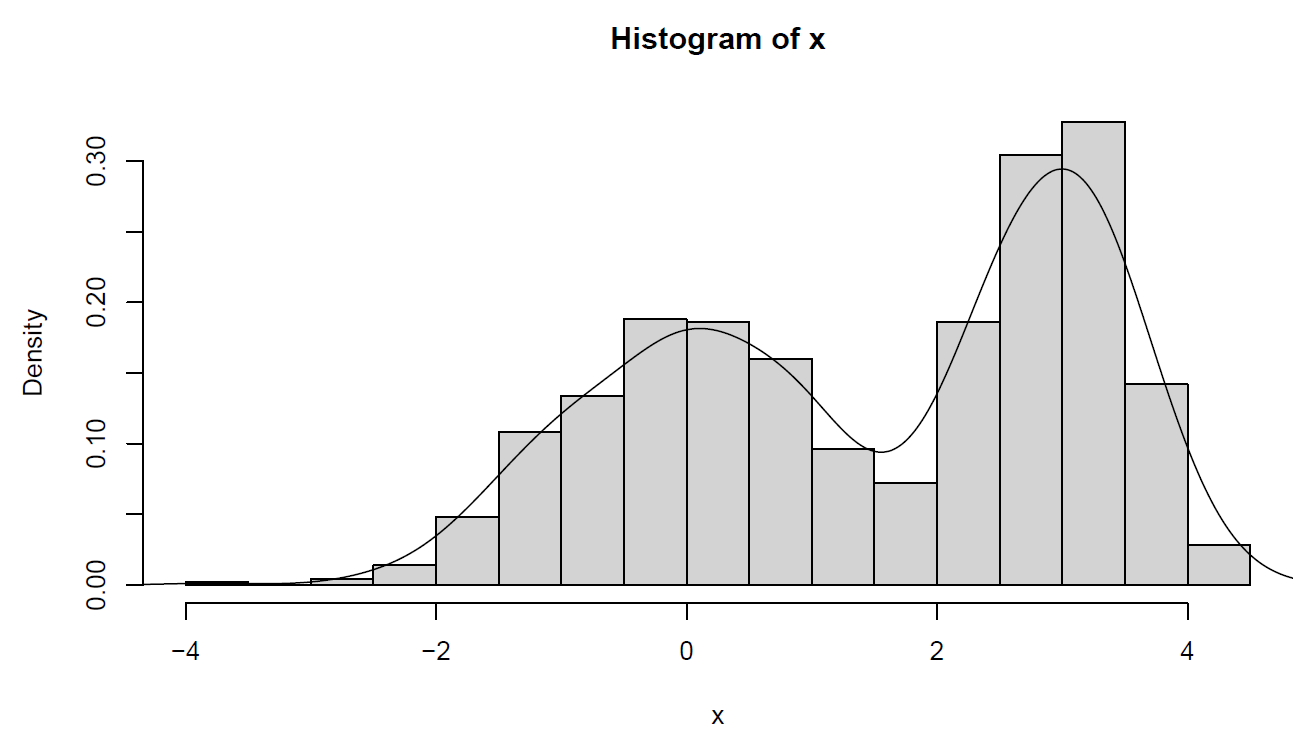
\includegraphics[width =0.7\textwidth]{figure_man/mixdist.png}
\end{center}

%<<echo = FALSE, out.width='80%', align='center'>>=
%n = 1000
%x1 = rnorm(n, 0, 1)
%x2 = rnorm(n, 3, 0.5)

%u = runif(1000)
%k = as.integer(u > 0.5)
%x = k * x1 + (1 - k) * x2

%hist(x, freq=FALSE, breaks=25)
%lines(density(x))
%@
\end{vbframe}

\begin{vbframe}{Sampling Multivariate gaussian}
$X=(X_1, ..., X_d) \sim N_d(\muv, \Sigma)$:
$$
f(x) = \frac{1}{(2\pi)^{d/2} |\Sigma|^{1/2}}exp(-\frac{1}{2}(\bm{x}-\muv)^T\Sigma^{-1}(\bm{x}-\muv))
$$
with mean $\muv=(\mu_1,...,\mu_d)^T$ and symmetrical, positive definite covariance matrix $\Sigma$.

\lz

\textbf{Sampling from multivariate Gaussian:}

\lz
\begin{enumerate}
\item Generate $Z=(Z_1,...,Z_d)$, with $Z_i \stackrel{iid}{\sim} N(0,1)$.
\item Transform random vector $Z$ to desired mean and covariance.
\end{enumerate}

\framebreak

\textbf{Derivation of Transformation:}

\lz

\begin{itemize}
\item If $Z \sim N_d(\muv, \Sigma)$, then $CZ+\bm{b}$ is $\sim N_d(C\muv+\bm{b}, C\Sigma C^T)$.

\lz

\item If $Z \sim N_d(0,\id_d)$, then $CZ+\bm{b}$ is $\sim N_d(\bm{b}, CC^T)$.

\lz

\item Assuming $\Sigma$ can be factorized into $\Sigma=CC^T$ for a matrix $C$, then $CZ+\muv \sim N_d(\muv, \Sigma)$.

\lz

\item Hence, $CZ+\muv$ is the transformation we are looking for.
\end{itemize}

\framebreak
\begin{itemize}
\item Calculation of the square root $\Sigma^{1/2}=C$ by \textbf{spectral decomposition}.

\lz

\item $\Sigma=P\Lambda P^{-1},$ with $\Lambda$ being a diagonal matrix of the eigenvalues of $\Sigma$ and $P$ being a matrix with the orthogonal eigenvectors in the columns space ($P^{-1}=P^T$).

\lz

\item $\Sigma^{1/2}$ then corresponds to $\Sigma^{1/2}=P\Lambda^{1/2} P^{-1}$, with $\Lambda^{1/2}=diag(\lambda_1^{1/2},..., \lambda_d^{1/2})$.

\lz

\item There are other possibilities to factorize $\Sigma$ (e.g. Cholesky decomposition) $\to$ see chapter 7.
\end{itemize}
\framebreak

\lz 

\begin{center}
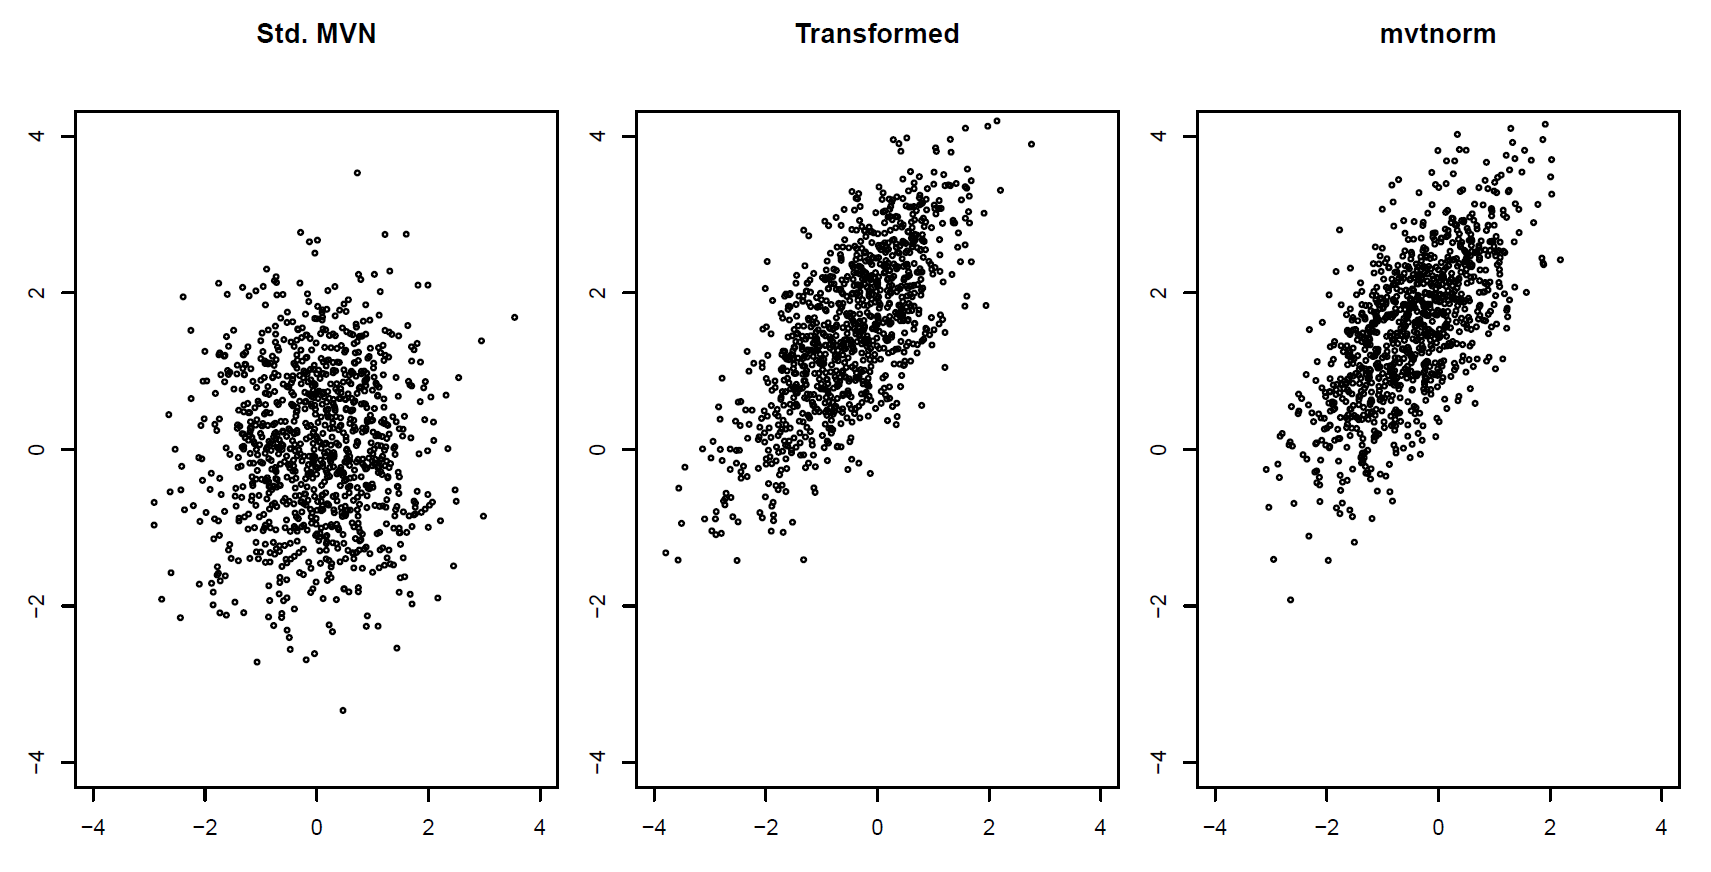
\includegraphics[width =1\textwidth]{figure_man/multigaussian.png}
\end{center}
%<<warning=FALSE, echo = FALSE>>=
%# Generate n = 1000 random vectors from MVN(mu, Sigma)
%n = 1000
%mu = c(-0.5, 1.5)
%Sigma = matrix(c(1, 0.7, 0.7, 1), ncol = 2, byrow = TRUE)
%d = length(mu)
%Z = matrix(rnorm(n * d), nrow = n, ncol = d)

%ev = eigen(Sigma, symmetric = TRUE)
%lambda = ev$values
%V = ev$vectors
%Q = V %*% diag(sqrt(lambda)) %*% t(V)
%X = Z %*% Q + matrix(mu, n, d, byrow = TRUE)

%# For comparison drawing from MVN with package mvtnorm
%library(mvtnorm)
%rmv <- rmvnorm(n, mu, Sigma)
%@
%<<echo=FALSE>>=
%par(mfrow=c(1,3), mar=c(6, 2, 6, 1))
%plot(Z[, 1], Z[, 2], xlim = c(-4,4), ylim = c(-4,4),
%     cex = 0.5, main = "Std. MVN", xlab="", ylab="")
%plot(X[, 1], X[, 2], xlim = c(-4,4), ylim = c(-4,4),
%     cex = 0.5, main = "Transformed", xlab="", ylab="")
%plot(rmv[,1], rmv[,2], xlim = c(-4,4), ylim = c(-4,4),
%     cex = 0.5, main = "mvtnorm", xlab="", ylab="")
%@
\end{vbframe}


% \begin{vbframe}{Vergleich der Performance von Zufallsgeneratoren}
% Existenz verschiedener Methoden für gegebene Verteilungen: Welche ist zu bevorzugen?
%
% \lz
%
% \begin{itemize}
% \item Laufzeit für Sampling
% \lz
% \item Varianz eines Schätzers aus gezogenen Zufallszahlen
% \end{itemize}
%
% % <<warning=FALSE, message=FALSE, size="scriptsize">>=
% % library(mvtnorm)
% % n <- 100          #sample size
% % d <- 30           #dimension
% % N <- 2000         #iterations
% % mu <- numeric(d)
% % system.time(for (i in 1:N)
% %     rmvnorm(n, mu, cov(matrix(rnorm(n*d), n, d)),
% %             method = c("eigen")))
% % system.time(for (i in 1:N)
% %     rmvnorm(n, mu, cov(matrix(rnorm(n*d), n, d)),
% %             method = c("chol")))
% % @
% \end{vbframe}


\endlecture
\end{document}